
%%
%% This .tex file is for use with BibLaTeX.
%%
%% As of Spring 2023, the School of Graduate Studies requires some minimum accessibility requirements for all electronic theses. Accessibility is difficult to produce with LaTeX on the front end, but fortunately it is quite easy to meet the requirements on the back end using Adobe (not Adobe Reader). Simply download the PDF of your thesis and follow this guide: https://case.edu/gradstudies/sites/case.edu.gradstudies/files/2023-02/CWRU%20Thesis%20and%20Dissertation%20Accessiblity%20Guide_0.pdf
%%%%%%%%%%%%

\documentclass[12pt]{cwru_thesis}
\usepackage[hyphens]{url}
\usepackage{indentfirst}
\usepackage{lipsum}
\usepackage{tabularx}
\usepackage{graphicx}
\usepackage{hyperref}
\hypersetup{colorlinks=true, linkcolor=black, filecolor=black, urlcolor=black, citecolor=black}
\urlstyle{same}
% \usepackage[acronym,toc]{glossaries}
\usepackage[intoc]{nomencl}
\renewcommand{\nomname}{List of Symbols}

\usepackage{mathptmx}
\usepackage[T1]{fontenc}
\usepackage[utf8]{inputenc}
\usepackage{amsfonts, amsmath, amsthm, amssymb}


\newcommand{\dif}{\mathrm{d}}
\newcommand{\Dif}{\mathrm{D}}
\renewcommand{\vec}[1]{\ensuremath{\underline{#1}}}
\newcommand{\grad}{\underline{\nabla}}
\newcommand{\curl}{\underline{\nabla} \times}
\newcommand{\lap}{\underline{\nabla}^2}
\renewcommand{\div}{\underline{\nabla} \cdot}
\newcommand{\paren}[1]{\left( {#1} \right)}
\newcommand{\norm}[1]{\lVert#1\rVert}

% Must use biblatex to produce the Published Contents and Contributions, per-chapter bibliography (if desired), etc.
\usepackage[
    backend=biber,natbib,style=numeric-comp,maxbibnames=99
]{biblatex}

% Name of your .bib file(s)
\addbibresource{example.bib}

% \makeglossaries
%%%%%%%%%%%%%%%%%%%%%%%%%%%%%%%%%%%%%%%%%%%%%%%%%%%%%%%%%%%%%%%%%%%%%%%%%%%%%%%%%%%%%%%
%Glossary entries


%Acronyms to include in the list of acronyms
% \newacronym{mda}{MDA}{Multipath Discovery Algorithm}
% \newacronym{mca}{MCA}{Multipath Classification Algorithm}

\begin{document}
\pagenumbering{roman}

% Do remember to remove the square brackets!
\title{Omar's Thesis} %Title of your thesis in title case
\author{Omar Loudghiri} %Your name

\degreeaward{Master's of Science in Computer Science}                 % Degree to be awarded
\department{Department of Computer Science and Data Science}
\university{Case Western Reserve University}    % Institution name  
\unilogo{cwru_logo.eps}                                 % Institution logo
\defendmonth{August, 2024}          % Graduation month and year
\defenddate{July 10th, 2024}          % Date of thesis defense

%Committee Member names. If you have a different number of committee members for your defense, you will need to edit lines 183-190 of cwru_thesis.cls accordingly.
\committeeChair{An Wang} %Committee Chair's name
\committeeOne{Mark Allman} %Committee member #1's name
\committeeTwo{Vincenzo Liberatore} %Committee member #2's name
\committeeThree{Mehmet Koyuturk} %Committee member #3's name

%%  If you'd like to add the CWRU logo from your title page, simply add the "[logo]" text to the maketitle command. Note that the School of Graduate Studies doesn't like this.
\maketitle

\begin{dedication} 	 
  TBD
\end{dedication}

\begin{KeepFromToc}
  \tableofcontents
\end{KeepFromToc}
\listoftables
\listoffigures



\begin{acknowledgements}
   TBD
\end{acknowledgements}

%If you have acroynms you wish to define, include this line. If not, you may delete it. See https://www.overleaf.com/learn/latex/Glossaries#Acronyms for more information about how to use Acronyms.

% \printglossary[type=\acronymtype, title=List of Abbreviations]

%If you have terms you wish to define in a glossary, include this line. If not, you may delete it. See https://www.overleaf.com/learn/latex/Glossaries for more information about how to use Glossaries
% \printglossary

%If you have a nomenclature section for defining symbols, include this line. If not, you may delete it. See https://www.overleaf.com/learn/latex/Nomenclatures for more information about how to use Nomenclatures
\printnomenclature

\begin{abstract}
  TBD
\end{abstract}

\mainmatter

\setcounter{secnumdepth}{2}

\chapter{Introduction} 
\label{chap:intro}
Networks are fundamental to modern society, enabling communication, commerce, and data exchange. These networks are built from an array of user devices, routers, and servers. Understanding the architecture and dynamics of these networks is crucial for enhancing their efficiency and reliability. Research has long focused on mapping and analyzing network structures to improve their performance and resilience (Paxson, 1996). A key aspect of network optimization is load balancing, a practice employed by network operators to manage traffic distribution and scale network capacity. Keeping a current understanding of both network structures and load balancing techniques is essential for maintaining robust and efficient network operations.

Load balancing is a critical network management technique that distributes traffic across multiple servers or network paths. A load balancer is a piece of network equipment that can direct packets to one of several available routes, anticipating that each route will yield a similar result. This distribution helps prevent any single server from becoming overwhelmed and ensures efficient use of network resources.

Originally developed as network-based hardware, load balancing now often functions within routers. It plays a crucial role in modern infrastructure by ensuring high availability, scalability, security, and performance. Applications today must handle millions of simultaneous sessions, and load balancers dynamically distribute this traffic across servers with duplicate data, ensuring reliable and fast data delivery. This process can also provide redundancy; if a server fails, traffic may be redirected to maintain continuous access.

Load balancing has several benefits, including enhancing security by potentially minimizing attack surfaces and rerouting traffic if a server is compromised. It also optimizes performance by managing resource use and traffic spikes. Various algorithms, such as round-robin and least connections, help distribute traffic based on real-time conditions. However, it is important to note that load balancing itself can become a single point of failure if the load balancer goes down.

\section{Project Motivation and Goals}

The primary motivation for this project is to quantify the prevalence and characteristics of load balancing in the Internet. By measuring load balancing behavior and mapping the presence of load balancers across commonly used paths in the Internet, this research aims to enhance our understanding of their impact. The project focuses on identifying and categorizing load balancers, analyzing their deployment, and understanding the resulting network paths and their implications for the broader Internet infrastructure.

\section{Impact of Load Balancing on Internet Reliability}

Load balancing significantly enhances the reliability of the Internet by distributing traffic across multiple servers or paths. This helps prevent any single point of failure, manage high traffic volumes, and ensure continuous availability of services. Effective load balancing reduces latency, avoids downtime, and ensures smooth data delivery, contributing to a better user experience.

The primary motivation for this project is to explore how load balancing impacts Internet reliability. Understanding this impact is crucial, as load balancing directly affects the network's ability to handle failures, traffic spikes, and varying load conditions. Despite its importance, the extent of load balancing's contribution to Internet reliability has not been extensively quantified.

This research aims to measure and analyze the role of load balancing in maintaining Internet reliability. By mapping the global presence of load balancers and characterizing their behavior, we seek to provide a clearer picture of their impact on network resilience. Using tools like the Multipath Detection Algorithm (MDA), we will quantify how load balancing affects network performance.

In summary, load balancing is key to Internet reliability, and this project aims to quantify its significance.



\section{Areas of Study} \label{sec:Areassection}





% \subsection{This is a Subsection} \label{subsec:exsubsec}







\chapter{Related Works}

In \cite{Augustin2007}, Augustin et al. present a comprehensive study on load-balanced paths, highlighting the significance of recognizing load balancing in contemporary networking by demonstrating how it affects traffic distribution and path diversity. Our goal is to update the community's understanding of load balancing in the Internet 17 years after \cite{Augustin2007} was published.

The authors enhanced a traceroute-like tool called Paris traceroute, designed to find all paths between a pair of hosts. Their methodology involves identifying load-balancing routers and characterizing the load-balanced paths. By conducting measurements from 15 sources to over 68,000 destinations, their study reveals that the traditional single-path concept no longer holds. They found that 39\% of source-destination pairs traverse a load balancer, and this percentage rises to 70\% when considering paths between a source and a destination network.

This study was significant in showing the prevalence of load balancers. The insights gained from this work are critical for developing more realistic network models and improving the design and reliability of Internet applications.

\section{Traceroute}

Traceroute is a network diagnostic tool used to track the path packets take from one IP address to another. It works by sending packets with gradually increasing time-to-live (TTL) values. Each router along the path decreases the TTL of the packet by one. When the TTL reaches zero, the router sends back an error message to the sender, revealing its IP address. This process is repeated with incrementing TTL values, allowing traceroute to map out the entire route to the destination.

Traceroute provides insights into the structure and behavior of the network by identifying each hop along the route. However, traditional traceroute may not handle load-balanced paths well, as it can be misled by the varying paths packets may take. To address this, Paris traceroute and MDA are used to obtain more accurate measurements by maintaining consistent flow identifiers, thus avoiding misinterpretation caused by load balancers.

\section{Multipath Detection Algorithm (MDA)}

The Multipath Detection Algorithm (MDA) is a key component of Paris traceroute, designed to identify and trace multiple load-balanced paths between a source and a destination. Traditional traceroute tools often fail to detect load balancing because they assume a single path. In contrast, MDA systematically discovers all paths by varying flow identifiers in probe packets.

The MDA operates hop-by-hop, sending probes to identify all interfaces at each hop. For a given interface \(r\) at hop \(h-1\), MDA generates several flow identifiers to ensure probes reach \(r\). It then sends these probes one hop further to discover the next-hop interfaces \(s_1, s_2, \ldots, s_n\).

To determine the number of probes \(k\) needed to discover all paths with a high degree of confidence, MDA assumes \(r\) is part of a load balancer that splits traffic evenly across \(n\) paths. If fewer than \(n\) interfaces are found, MDA stops. Otherwise, it increases \(n\) and sends additional probes to test the hypothesis.

To identify whether a load balancer uses per-packet or per-flow balancing, MDA sends probes with a constant flow identifier. If responses come from multiple interfaces, it indicates per-packet balancing. If all responses come from the same interface, it suggests per-flow balancing. MDA uses statistical methods to ensure a high level of confidence (typically 95\%) in its classification.

For instance, to reject the hypothesis of \(n = 2\) with 95\% confidence, MDA sends \(k = 6\) probes. If load balancing across up to 16 interfaces is suspected, MDA may send up to \(k = 96\) probes to ensure all paths are discovered. This process allows MDA to effectively enumerate all paths and classify the type of load balancing in use.

\section{Usage of Paris Traceroute}

The paper by Augustin et al. \cite{Augustin2007} is one of the few studies that actively measures the presence and behavior of load balancers in the Internet. Although their work provides a strong foundation, further investigation is needed to account for the evolving nature of Internet infrastructure and load balancing techniques.

Building on the foundational work of Augustin et al., this research aims to further explore the presence and behavior of load balancers in the Internet. By leveraging Paris traceroute and its MDA, we conduct extensive measurements to map the global distribution of load balancers and analyze their impact on network performance and reliability.



This study will add to the existing knowledge by:
\begin{itemize}
    \item Including a diverse set of source-destination pairs.
    \item Investigating the effects of load balancing on different types of network traffic and applications.
\end{itemize}

\section{Scamper}

\subsection{Introduction}

Packet probing experiments capture simple measurements—typically delay, loss, reordering, and topology—that provide valuable insights into the structure and behavior of the Internet. For instance, early studies on packet size and delay led to improvements in the TCP RTO algorithm. As the Internet has grown, measuring it has become more complex, both technically and methodologically. Over the past decade, researchers have developed and operated many large-scale Internet measurement platforms, each involving significant software development.

In 2005, facing funding challenges, the Internet measurement community organized a workshop to plan a collaborative, community-oriented network measurement infrastructure. The workshop report highlighted the need for better organization of large-scale measurements.

This paper addresses a small part of this problem by focusing on building a packet-prober for large-scale measurements and well-defined data archiving. A packet-prober should simplify the coordination of measurements, provide APIs for operating system differences, offer accurate timing information, and produce detailed, easy-to-process output. This approach helps researchers avoid system programming and administrative challenges, allowing them to implement new measurement techniques and focus on analysis and validation.

\subsection{Scamper Features}

Scamper is a powerful packet-prober designed to support large-scale Internet measurement. It includes feature-rich implementations of traceroute, ping, MDA traceroute, four alias resolution techniques, Sting, and parts of TBIT.

\subsection{Multipath Detection Algorithm (MDA) in Scamper}

Scamper implements the Multipath Detection Algorithm (MDA) described by Augustin et al. to infer all interfaces visited between a source and destination in a per-flow load-balanced Internet path. MDA achieves this by deliberately varying the flow identifier that a router may compute when load balancing. Probes with different flow identifiers may take different paths, thereby revealing different parts of the forward IP path.

In addition to the ICMP and UDP methods originally implemented by Augustin et al., which vary the ICMP checksum and UDP destination port values, Scamper implements a UDP method that varies the source port instead of the destination port. This prevents the probes from appearing as a port scan and enables probing past firewalls that block UDP probes to ports above the usual range used by traceroute. Scamper also implements TCP methods that vary the flow identifier by changing either the source or destination port, depending on the user’s choice.

Scamper's MDA traceroute functionality was used to conduct scheduled data collection throughout this project.

\section{Classification of Load Balancing in the Internet and Multipath Classification Algorithm (MCA)}

Recent advances in programmable data planes, software-defined networking, and the adoption of IPv6 have enabled more complex load balancing strategies. Almeida et al. introduced the Multipath Classification Algorithm (MCA), which enhances the existing Multipath Detection Algorithm (MDA). While MDA systematically varies probes' flow identifiers to identify load-balanced paths, MCA extends this by considering arbitrary combinations of bits in the packet header for load balancing.

The key contributions of MCA include:
\begin{itemize}
    \item \textbf{Enhanced Classification:} MCA identifies the specific bits in the packet header used by load balancers, providing a more detailed and accurate classification than MDA, which primarily varies transport port numbers and the ICMP checksum.
    \item \textbf{Efficiency Optimizations:} The researchers developed optimizations to reduce the probing cost. MCA achieves this with a modest increase in the number of probes, only 34\% higher than MDA, while maintaining accuracy.
    \item \textbf{Comprehensive Measurements:} Through large-scale measurement campaigns, MCA characterizes load balancing on both IPv4 and IPv6 Internet paths. The results show that load balancing is more prevalent and sophisticated than previously reported.
\end{itemize}

The study revealed that 74\% of IPv4 and 56\% of IPv6 routes traverse at least one load balancer. Additionally, 23\% of IPv4 and 18\% of IPv6 load balancers have three or more next hops, indicating complex load balancing configurations.

Building on this work, part of our research uses MCA to map the global presence of load balancers and analyze their impact on network performance and reliability. In the next section, we will discuss how MDA and MCA were integrated into our research and the rationale behind choosing these methodologies.

\section{MDA vs MCA}

While MCA offers significant improvements in identifying and classifying load balancers by considering a broader range of packet header bits, it is less accessible for fine-tuning and practical use. For our research, we opted to use MDA due to its better integrability with existing tools and faster runtime performance. MDA's established methodologies and ease of implementation make it a more practical choice for large-scale measurements. The decision to use MDA is further justified by its compatibility with current infrastructure and the ability to conduct measurements efficiently. 
\chapter{Methodology}

This chapter details the methods used to collect and analyze data for detecting and characterizing load balancers in network paths. We employed two lists derived from the Alexa Top 1 Million Websites list and performed Paris traceroute measurements to these hostnames. The collected data was then processed to identify load balancers and analyze their behavior.

\section{Background Information}

The Alexa Top 1 Million Websites list was used to obtain hostnames for our study. Additionally, the Team Cymru IP to ASN mapping service was utilized to resolve IP addresses to their corresponding Autonomous System Numbers (ASNs). These lists and tools provided the necessary foundation for our analysis.

\subsection{Alexa Top 1 Million Websites}

The Alexa Top 1 Million Websites list was utilized to obtain hostnames for this research. A current version of the Alexa list was obtained when we started our data collection in February 2023. The Alexa list is widely used in network measurement studies due to its popularity, even though it is not known for high accuracy, particularly for lower-ranked sites \cite{Alexa}.

For our study, we took two different subsets of this list:
\begin{itemize}
    \item The top 2000 websites.
    \item A random selection of 2000 websites from the top 100,000 sites.
\end{itemize}
These subsets allowed us to collect a diverse set of data through Paris traceroute runs to the selected hostnames.

\subsection{Team Cymru IP to ASN List}

For this project, the Team Cymru IP to ASN mapping service was utilized to resolve IP addresses to their corresponding Autonomous System Numbers (ASNs). Team Cymru provides a service dedicated to mapping IP numbers to BGP prefixes and ASNs, based on BGP feeds from over 50 peers, updated at four-hour intervals \cite{Cymru}.

In this project, the Team Cymru service was essential for mapping IP addresses to ASNs. We collected ASN-to-IPv4 address information from Team Cymru every month, with their permission. This list was used to cross-reference the IPs identified as load balancers, their next hops, and their destination IPs, providing detailed insights into the load balancers discovered.

Here is an example of an entry with definitions of the fields:
\begin{table}[h]
    \centering
    \begin{tabular}{|l|l|}
        \hline
        \textbf{Field} & \textbf{Example} \\
        \hline
        BGP Origin ASN & 23489 \\
        \hline
        BGP Peer ASN & 199.88.100.1 \\
        \hline
        BGP Prefix & 199.88.100.0/24 \\
        \hline
        Prefix Country Code (assigned) & US \\
        \hline
        Prefix Registry (assigned) & arin \\
        \hline
        Prefix Allocation Date & 1994-03-28 \\
        \hline
        ASN Country Code (assigned) & US \\
        \hline
        ASN Registry (assigned) & arin \\
        \hline
        ASN Allocation Date & 1994-03-28 \\
        \hline
        ASN Description & MARINK12, US \\
        \hline
    \end{tabular}
    \caption{BGP and ASN Information}
    \label{tab:bgp_asn_info}
\end{table}

\section{Discovering Load Balancers}

The primary objective of this research is to record the paths between our vantage point and a set of popular hosts, and to detect and characterize load balancers along these paths. To achieve this, we used two distinct lists obtained from the Alexa Top 1 Million Websites list.

\subsection{Measurement Frequency and Timeline}

To ensure the feasibility of daily measurements, 2000 IP addresses were chosen for the Paris traceroute process. Each IP takes an average of 40 seconds to return a complete trace with load balancer information. This duration allows the script to run through 2000 IPs in approximately 23 hours, making it possible to conduct measurements on a daily basis.

The goal of daily measurements is to assess trends and variations in load balancing behavior over time. To maintain feasibility, we alternated between the Top-2000 list and the Rand-2000 list each day. This rotation allowed us to gather comprehensive data while managing the logistical constraints of daily measurements.

The measurements were run continuously from January 23, 2024, to April 16, 2024, on a Linux machine at the International Computer Science Institute (ICSI) in Berkeley, CA. This timeline ensured the collection of extensive data over several months, capturing potential variations and trends in load balancing behavior and network topology over time.

\subsection{IP Lists}

Two distinct lists were used for this study:
\begin{itemize}
    \item \textbf{Top-2000 List:} This list includes the top 2000 domains from the Alexa list. It is designed to cover an important chunk of the most used websites around the Internet, ensuring that the analysis captures the behavior and infrastructure of significant routes.
    \item \textbf{Rand-2000 List:} This list comprises 2000 random domains selected from the top 100,000 websites on the Alexa list, with a new random selection made each time we ran the measurement. It aims to provide a well-rounded analysis of the Internet's topology by including popular but not exclusively top-ranked sites.
\end{itemize}

Using the top 2000 websites allows us to measure load balancers on sites that are heavily accessed, providing insights into the infrastructure of widely used services. The random selection of 2000 sites from the top 100,000 ensures a broader view of the Internet's topology, capturing data from a diverse set of sites.



\section{Data Analysis}

The data analysis process involved systematically processing and analyzing our collected traceroute data. This analysis aimed to identify and categorize load balancers, as well as to visualize the results effectively.

\subsection{Paris Traceroute on IP Lists}

For each domain in the Rand-2000 and Top-2000 lists, the Paris traceroute tool was used with the Multipath Detection Algorithm (MDA) to conduct traceroute measurements. The IP to ASN mapping service was then used to resolve IP addresses to their corresponding Autonomous System Numbers (ASNs). This information was used to cross-reference the IPs identified as load balancers, their next hops, and their destination IPs.

\subsection{Counting Matches and Mismatches of Next Hop AS}

The next part of the analysis involved counting how often the AS of a next hop matched or mismatched the AS of the load balancer. This step aimed to understand the distribution of next hops in relation to their associated load balancers. This analysis provided a detailed view of the relationships between load balancers and their next hops.

\subsection{Characterizing Next Hop Counts}

To gain further insights into the behavior of load balancers, the number of next hops for each load balancer was analyzed. The mean, median, and mode of the next hop counts were calculated to summarize the distribution. This analysis helped characterize the diversity of paths taken by traffic after passing through load balancers.

\subsection{Identifying Top Load Balancer Groups}

Finally, the analysis identified the top load balancer groups based on the number of domains they served. By examining the number of domains associated with each load balancer, we were able to determine the most significant load balancer groups. The results highlighted the most prominent load balancers, showing which load balancers serve the highest number of domains.

\subsection{Finding Common Next Hops Across Domains}

The analysis started with identifying common next hops shared by multiple load balancers across different domains. The first step was loading the mapping of destinations to load balancers and their next hops from the data. Additionally, AS information for IPs was loaded to provide context for the identified next hops. 

The analysis focused on finding next hops that were common to at least three load balancers across different domains. The results provided insights into common paths used by different domains, highlighting shared infrastructure.

\chapter{Topography of Load Balancers}

In this chapter, we examine the distribution and prevalence of load balancers across two different datasets resulting from two distinct lists: the Top-2000 and the Rand-2000. By analyzing these datasets, we aim to understand how load balancers are utilized in the infrastructure of popular and randomly selected websites.

\section{Analysis of Load Balancer Distribution}

\subsection{Top-2000 Dataset}

The Top-2000 dataset consists of 117 days of data collected between November 9, 2023, and April 16, 2024. During this period, the number of domains with at least one load balancer ranged from a minimum of 279 to a maximum of 1680. The average number of domains with load balancers was 1644.08, indicating that 82.2\% of the paths to these top domains include load balancers. The median value of 1668 further supports the observation that the majority of these domains consistently use load balancers, highlighting the importance of load balancing in maintaining the reliability and performance of high-traffic websites.

The minimum of 279 is about one-sixth of the median, suggesting significant variability. This could be due to measurement errors or temporary changes in the network paths. Investigating these anomalies could provide further insights into the consistency and reliability of load balancer detection.

\subsection{Rand-2000 Dataset}

The Rand-2000 dataset includes 112 days of data collected over the same period, from November 9, 2023, to April 16, 2024. The number of domains with at least one load balancer in this dataset varied between 1205 and 1297. The average number of domains with load balancers was 1251.29, with a median of 1252. These statistics show that 62.5\% of the paths to these randomly selected domains include load balancers, indicating a substantial use of load balancers across a diverse set of websites.

\subsection{Comparison and Insights}

The scatter plot in Figure \ref{fig:scatter_plot_domains} illustrates the number of domains with at least one load balancer over time for both the Top-2000 and Rand-2000 datasets. This visual representation shows that the number of detected load balancers is relatively constant over the measurement period.

\begin{figure}[h]
    \centering
    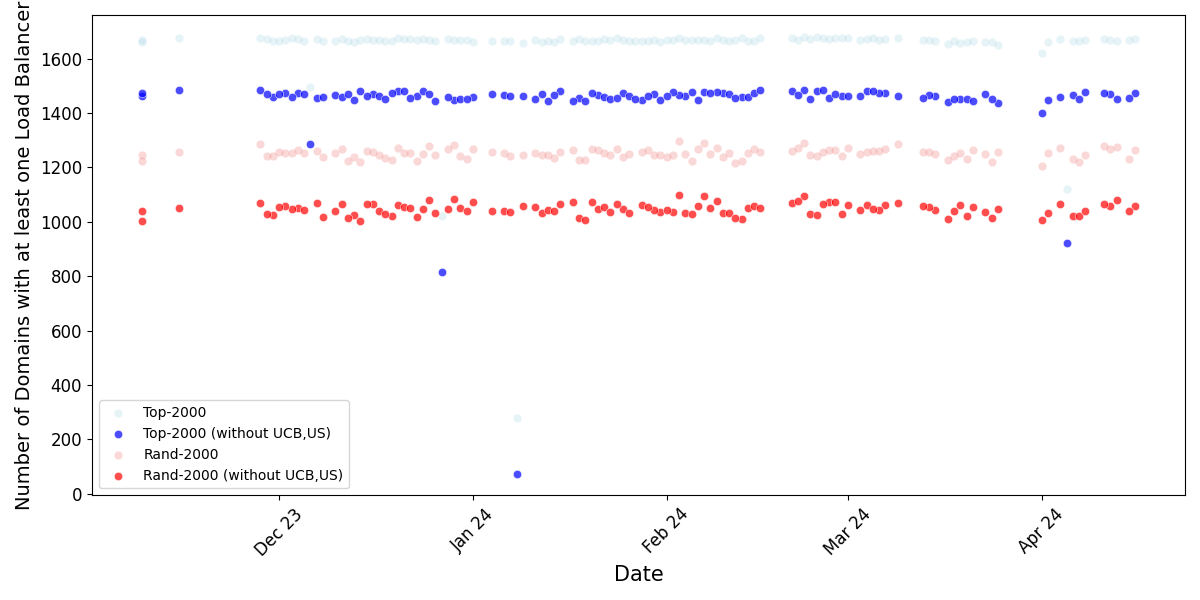
\includegraphics[width=\textwidth]{figures/scatter_plot_domains.png}
    \caption{Number of Domains with at least one Load Balancer Over Time}
    \label{fig:scatter_plot_domains}
\end{figure}

The higher average and median values in the Top-2000 dataset underscore the higher usage of load balancers in managing traffic for the most visited websites. These sites likely experience higher and more variable traffic, necessitating robust load balancing solutions to ensure uptime and performance. Meanwhile, the Rand-2000 dataset demonstrates that load balancing is also prevalent for a broad spectrum of domains.

\section{Analysis of Next Hops After Load Balancers}

We focused on understanding the behavior of next hops after load balancers. This analysis helps us gain insights into how load distribution is managed.

\subsection{Top-2000 Dataset}

The Top-2000 dataset consists of 192,357 load balancers. The analysis reveals that the number of next hops after a load balancer ranges from a minimum of 2 to a maximum of 102. The average number of next hops is approximately 3.90, indicating a moderate level of load distribution across multiple paths. The median value stands at 3.0, suggesting that half of the load balancers have three or fewer next hops. The standard deviation is 5.75, reflecting significant variability in the number of next hops. Furthermore, the 75th percentile is at 5.0, while the 95th percentile reaches 13.0, showing that a small number of load balancers have a high number of next hops.

\subsection{Rand-2000 Dataset}

In comparison, the Rand-2000 dataset includes 140,144 load balancers. Here, the number of next hops ranges from a minimum of 1 to a maximum of 25. The average number of next hops is 1.58, indicating a lower level of load distribution compared to the Top-2000 dataset. The median number of next hops is 1, suggesting that more than half of the load balancers have only one next hop. The standard deviation is 1.34, indicating less variability. The 75th percentile is 2.0, and the 95th percentile is 3.0, showing a more concentrated distribution of next hops.

\begin{figure}[h]
    \centering
    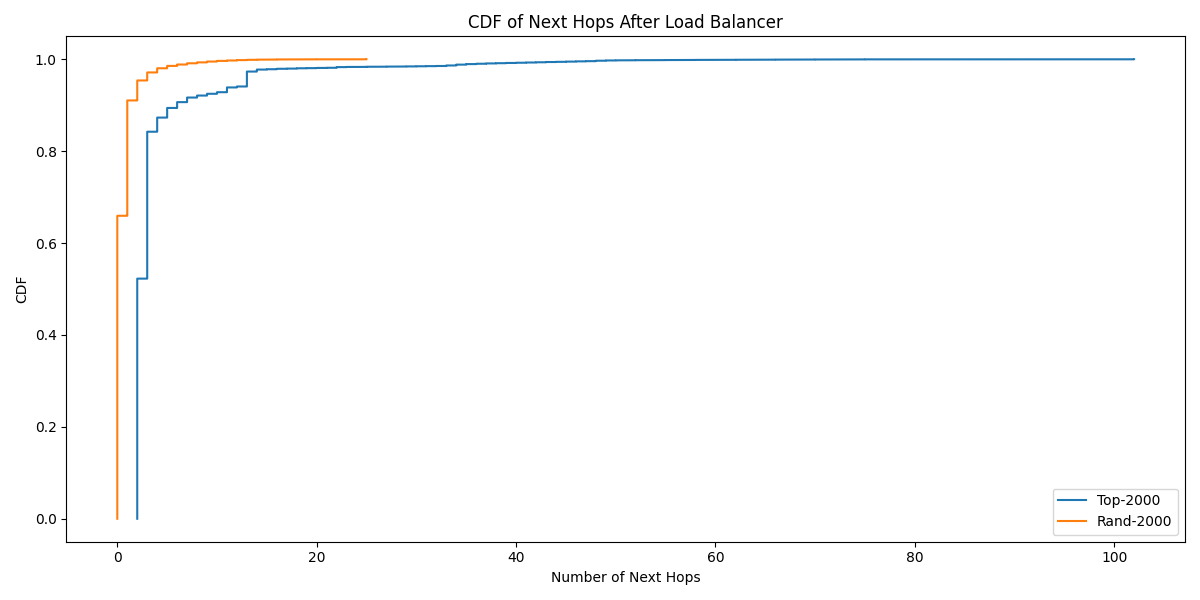
\includegraphics[width=\linewidth]{figures/cdf_next_hops.png}
    \caption{CDF of Next Hops After Load Balancers for Top-2000 and Rand-2000 Datasets}
    \label{fig:cdf_next_hops}
\end{figure}

Figure \ref{fig:cdf_next_hops} illustrates the cumulative distribution function (CDF) of the number of next hops after load balancers for both the Top-2000 and Rand-2000 datasets. The CDF provides a visual representation of the distribution and helps in comparing the two datasets. As shown, the Top-2000 dataset demonstrates a wider spread with more load balancers having a higher number of next hops, whereas the Rand-2000 dataset shows a more concentrated distribution with most load balancers having fewer next hops.



The differences in the number of next hops between the two datasets highlight the varying network configurations and load distribution strategies. The higher variability in the Top-2000 dataset suggests a more complex and distributed network structure. In contrast, the Rand-2000 dataset's lower variability and fewer next hops suggest a simpler network configuration for less commonly used paths.

\section{Analysis of ASes with Most Next Hops}

The analysis of Autonomous Systems (ASes) with the highest average number of next hops reveals significant insights into the infrastructure and load balancing requirements of these networks. The ASes with the most next hops typically indicate a robust infrastructure with a greater need for load balancing. This could be due to a high volume of traffic, requiring efficient distribution across multiple servers to avoid bottlenecks, or due to specific requirements such as traffic filtering based on the source.

The comparison between the Top-2000 and Rand-2000 datasets shows that the differences are not very significant, with similar ASes appearing across both lists. This suggests that the predominant load balancing providers are optimizing for scalability, redundancy, geographic distribution, application segmentation, resource optimization, and compliance. These factors are crucial for maintaining high performance, fault tolerance, and legal compliance in diverse geographical locations.

\begin{table}[h!]
    \centering
    \begin{tabularx}{\textwidth}{|X|r|}
        \hline
        \multicolumn{2}{|c|}{\textbf{Top 10 ASes by Average Number of Next Hops (Top-2000)}} \\
        \hline
        \textbf{AS} & \textbf{Average Next Hops} \\
        \hline
        ORACLE-BMC-31898, US & 90.69 \\
        FACEBOOK, US & 24.97 \\
        ADJUST-, DE & 24.16 \\
        CHINANET-SH-AP China Telecom Group, CN & 20.59 \\
        CHINA169-BJ China Unicom Beijing , CN & 19.82 \\
        CHINANET-BJ-AP, China Telecommunications, CN & 15.44 \\
        CLOUDFLARENET, US & 13.95 \\
        ALIBABA-CN-NET Alibaba Advertising , Ltd., CN & 13.89 \\
        CHINANET-SCIDC-AS-AP CHINANET SiChuan, CN & 13.82 \\
        CHINANET-BACKBONE No.31, Jin-rong Street, CN & 13.74 \\
        \hline
        \multicolumn{2}{|c|}{\textbf{Top 10 ASes by Average Number of Next Hops (Rand-2000)}} \\
        \hline
        \textbf{AS} & \textbf{Average Next Hops} \\
        \hline
        ORACLE-BMC-31898, US & 66.92 \\
        FACEBOOK, US & 17.88 \\
        ADJUST-, DE & 16.78 \\
        CHINANET-SH-AP China Telecom Group, CN & 15.20 \\
        CHINA169-BJ China Unicom Beijing, CN & 14.36 \\
        CHINANET-SCIDC-AS-AP CHINANET SiChuan, CN & 11.33 \\
        CLOUDFLARENET, US & 9.95 \\
        CHINANET-BACKBONE No.31, Jin-rong Street, CN & 9.78 \\
        CT-HANGZHOU-IDC No.288, Fu-chun Road, CN & 9.28 \\
        CHINANET-BJ-AP, China Telecommunications, CN & 9.20 \\
        \hline
    \end{tabularx}
    \caption{Top 10 ASes by Average Number of Next Hops for Top-2000 and Rand-2000}
    \label{tab:as_next_hops}
\end{table}

The presence of ASes such as ORACLE-BMC-31898, FACEBOOK, and various Chinese telecommunications providers across both datasets underscores the need for efficient load balancing in these networks. High average next hops could suggest various needs such as:
\begin{itemize}
    \item Optimization for scalability to handle large traffic volumes.
    \item Redundancy for fault tolerance.
    \item Geographic distribution for low-latency access.
    \item Compliance with data residency laws
\end{itemize} 

While this list is not exhaustive, these factors are critical in ensuring that no single server becomes a bottleneck, maintaining service continuity, and providing optimal performance to users in various regions. 


The similarities between the Top-2000 and Rand-2000 datasets indicate that these load balancing strategies are consistent across both high-traffic and more general websites, reflecting a broad application of these optimization techniques.


\section{Overall Analysis of Next Hop ASes Matches and Mismatches}

In our comprehensive analysis across all load balancers, we identified significant patterns in the matching and mismatching of next hops.

Our results revealed that out of a total of 192,357 load balancers analyzed in the Top-2000 dataset, and 140,144 load balancers in the Rand-2000 dataset, we observed a total of 104,214 unique load balancers. Among these, 80,979 were fully matching, where every next hop AS matched the load balancer AS, representing 77.7\% of the total unique load balancers. Fully matching next hops indicate a high degree of routing consistency within the AS.

Partially matching next hops, where at least one but not all next hops matched the load balancer AS, accounted for 402 instances, or 0.4\% of the total. These partial matches suggest a mixed routing strategy where some paths are optimized within the AS, while others diverge.

Next hops with no matching AS comprised 22,833 instances, making up 21.9\% of the total load balancers. This scenario points to significant routing divergence, potentially due to dynamic routing policies or external influences.

Figure~\ref{fig:overall_match_mismatch} illustrates the overall distribution of fully matching, partially matching, and no matching next hops. The pie chart provides a clear visual representation of the dominant patterns in next hop routing behavior.

\begin{figure}[h!]
    \centering
    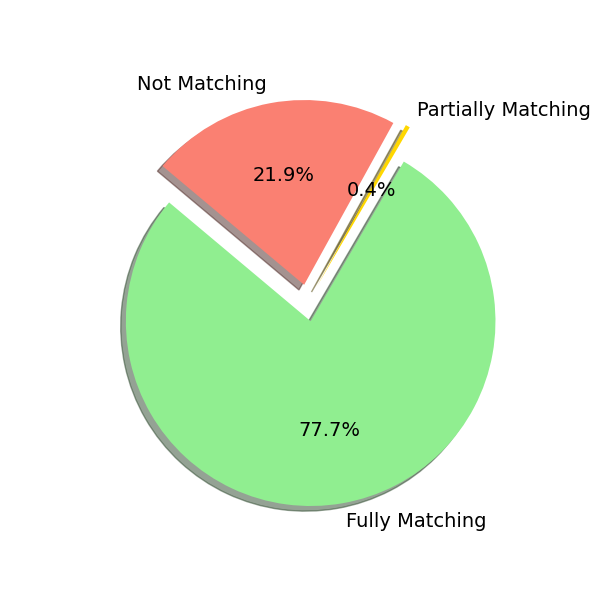
\includegraphics[width=\linewidth]{figures/overall_match_mismatch.png}
    \caption{Overall Load Balancer Next Hop Matching}
    \label{fig:overall_match_mismatch}
\end{figure}

\newpage
Our analysis also highlighted the top Autonomous Systems (ASes) based on the number of matches and mismatches. Table \ref{tab:match_mismatch} presents the top ASes in each category.

\begin{table}[h!]
    \centering
    \begin{tabular}{|l|r|}
        \hline
        \multicolumn{2}{|c|}{\textbf{Top 10 ASes with Fully Matching Next Hops}} \\
        \hline
        \textbf{AS} & \textbf{Count} \\
        \hline
        UCB, US & 30,890 \\
        Google, US & 13,516 \\
        ChinaNet Backbone No.31, Jin-Rong Street, CN & 6,420 \\
        Comcast-7922, US & 5,460 \\
        China169-BJ China Unicom Beijing Province Network, CN & 4,028 \\
        KDDI Corporation, JP & 3,204 \\
        Facebook, US & 2,321 \\
        Microsoft-Corp-MSN-AS-Block, US & 2,260 \\
        Cogent-174, US & 1,769 \\
        KIXS-AS-KR Korea Telecom, KR & 1,744 \\
        \hline
        \multicolumn{2}{|c|}{\textbf{Top 10 ASes with Partially Matching Next Hops}} \\
        \hline
        \textbf{AS} & \textbf{Count} \\
        \hline
        ChinaNet-IDC-BJ-AP IDC, China Telecommunications Corporation, CN & 158 \\
        ChinaNet Backbone No.31, Jin-Rong Street, CN & 125 \\
        RelianceJio-IN Reliance Jio Infocomm Limited, IN & 30 \\
        Yandex, RU & 18 \\
        GlobalDC, FI & 17 \\
        Level3, US & 15 \\
        NL-Gigapop, US & 12 \\
        HiNetUSA HiNet Service Center in U.S.A, TW & 12 \\
        Alibaba-CN-Net Hangzhou Alibaba Advertising Co., Ltd., CN & 4 \\
        Alibaba-CN-Net Alibaba US Technology Co., Ltd., CN & 4 \\
        \hline
        \multicolumn{2}{|c|}{\textbf{Top 10 ASes with No Matching Next Hops}} \\
        \hline
        \textbf{AS} & \textbf{Count} \\
        \hline
        CONE, US & 6,908 \\
        Domain\_AS & 5,580 \\
        UCB, US & 2,525 \\
        CSUNET-NW, US & 2,440 \\
        ChinaNet Backbone No.31, Jin-Rong Street, CN & 854 \\
        Level3, US & 849 \\
        Yahoo-1, US & 608 \\
        CSUNET-NE, US & 312 \\
        Google, US & 216 \\
        BTN-ASN, US & 207 \\
        \hline
    \end{tabular}
    \caption{Top 10 ASes with Fully Matching, Partially Matching, and No Matching Next Hops}
    \label{tab:match_mismatch}
\end{table}

\newpage

Overall, the findings suggest that while a majority of next hops maintain consistency within their ASes, there are notable instances of partial and no matches. This indicates that ASes mostly perform load balancing for their own nodes rather than for external nodes. This behavior makes sense because load balancing for external nodes would be costly without significant benefits to internal networks. However, the 22.3\% of non-matching load balancers is quite surprising. This could imply that load balancing from network providers or CDNs like Cloudflare is offered as a service, or it could suggest that there might be some inaccuracies in AS matching in certain cases.

UCB, US, is the local Autonomous System and therefore it is normal to find disproportionate amounts of load balancers belonging to it. The findings suggest that load balancing is predominantly done within the same AS, with very minute instances of overlap indicating that inter-AS load balancing is rare. This is likely due to the high costs associated with implementing such infrastructure and its primary use for managing load within the autonomous system itself rather than for external nodes.


\section{Change Over Time}

This section presents the statistics for the Top-2000 and Rand-2000 datasets, including the total number of days observed, the average daily changes, and the number of reappearances. Additionally, the top 5 most consistent and least consistent load balancers for both datasets are listed.

\subsection{Top-2000 Dataset}

Over the observation period of 116 days, an average of approximately 253.47 load balancers were added per day in the Top-2000 dataset. Conversely, an average of 251.21 load balancers were lost each day. The dataset also recorded a total of 82,318 reappearances, indicating the number of times load balancers reappeared after having been previously lost. The average duration of presence for a load balancer in this dataset was 31.10 days.

\begin{table}[h!]
    \centering
    \begin{tabular}{|l|l|}
        \hline
        \textbf{Most Consistent Load Balancers} & \textbf{Duration (days)} \\ \hline
        169.229.0.140 : UCB, US & 116 \\ \hline
        137.164.11.94 : CSUNET-NW, US & 116 \\ \hline
        157.240.81.224 : FACEBOOK, US & 116 \\ \hline
        157.240.112.88 : FACEBOOK, US & 116 \\ \hline
        129.134.118.175 : FACEBOOK, US & 116 \\ \hline
    \end{tabular}
    \caption{Top 5 Most Consistent Load Balancers in Top-2000 Dataset}
\end{table}

In contrast, the least consistent load balancers, each appearing for only a single day, are shown in the following table:

\begin{table}[h!]
    \centering
    \begin{tabular}{|l|l|}
        \hline
        \textbf{Least Consistent Load Balancers} & \textbf{Duration (days)} \\ \hline
        202.97.27.181 : CHINANET-BACKBONE, CN & 1 \\ \hline
        203.208.151.181 : SINGTEL-AS-AP, SG & 1 \\ \hline
        203.208.178.185 : SINGTEL-AS-AP, SG & 1 \\ \hline
        203.208.154.45 : SINGTEL-AS-AP, SG & 1 \\ \hline
        203.208.171.9 : SINGTEL-AS-AP, SG & 1 \\ \hline
    \end{tabular}
    \caption{Top 5 Least Consistent Load Balancers in Top-2000 Dataset}
\end{table}

\begin{figure}[h!]
    \centering
    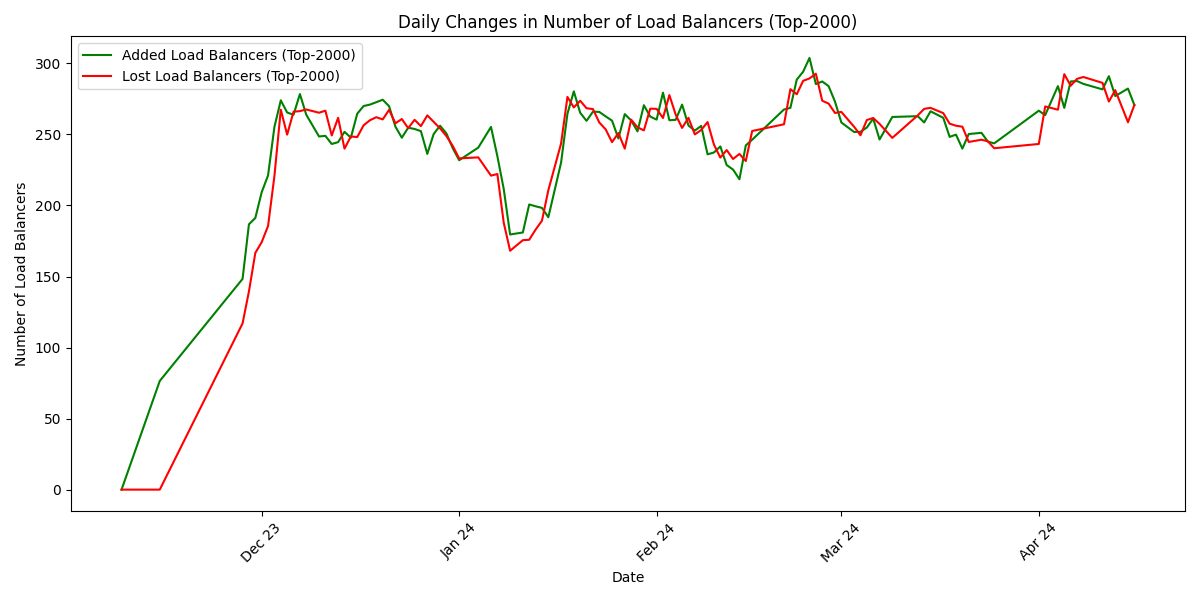
\includegraphics[width=\linewidth]{figures/load_balancer_changes_Top-2000.png}
    \caption{Daily Changes in Number of Load Balancers for Top-2000}
    \label{fig:top2000_changes}
\end{figure}

\subsection{Rand-2000 Dataset}

The Rand-2000 dataset, observed over 111 days, provided the following insights: On average, approximately 161.02 load balancers were added per day, while an average of 162.22 load balancers were lost each day. The dataset also recorded a total of 12,139 reappearances, highlighting the instances where load balancers reappeared after being lost. The average duration of presence for a load balancer in this dataset was 12.49 days.

\begin{table}[h!]
    \centering
    \begin{tabular}{|l|l|}
        \hline
        \textbf{Most Consistent Load Balancers} & \textbf{Duration (days)} \\ \hline
        169.229.0.140 : UCB, US & 111 \\ \hline
        137.164.11.94 : CSUNET-NW, US & 41 \\ \hline
        142.251.231.97 : GOOGLE, US & 40 \\ \hline
        142.251.231.99 : GOOGLE, US & 32 \\ \hline
        74.125.50.18 : GOOGLE, US & 30 \\ \hline
    \end{tabular}
    \caption{Top 5 Most Consistent Load Balancers in Rand-2000 Dataset}
\end{table}

The least consistent load balancers in the Rand-2000 dataset, each appearing for a single day, are shown below:

\begin{table}[h!]
    \centering
    \begin{tabular}{|l|l|}
        \hline
        \textbf{Least Consistent Load Balancers} & \textbf{Duration (days)} \\ \hline
        104.44.19.140 : MICROSOFT-CORP-MSN-AS-BLOCK, US & 1 \\ \hline
        104.44.18.166 : MICROSOFT-CORP-MSN-AS-BLOCK, US & 1 \\ \hline
        157.240.51.143 : FACEBOOK, US & 1 \\ \hline
        202.97.53.13 : CHINANET-BACKBONE, CN & 1 \\ \hline
        163.253.2.16 : INTERNET2-RESEARCH-EDU, US & 1 \\ \hline
    \end{tabular}
    \caption{Top 5 Least Consistent Load Balancers in Rand-2000 Dataset}
\end{table}

\begin{figure}[h!]
    \centering
    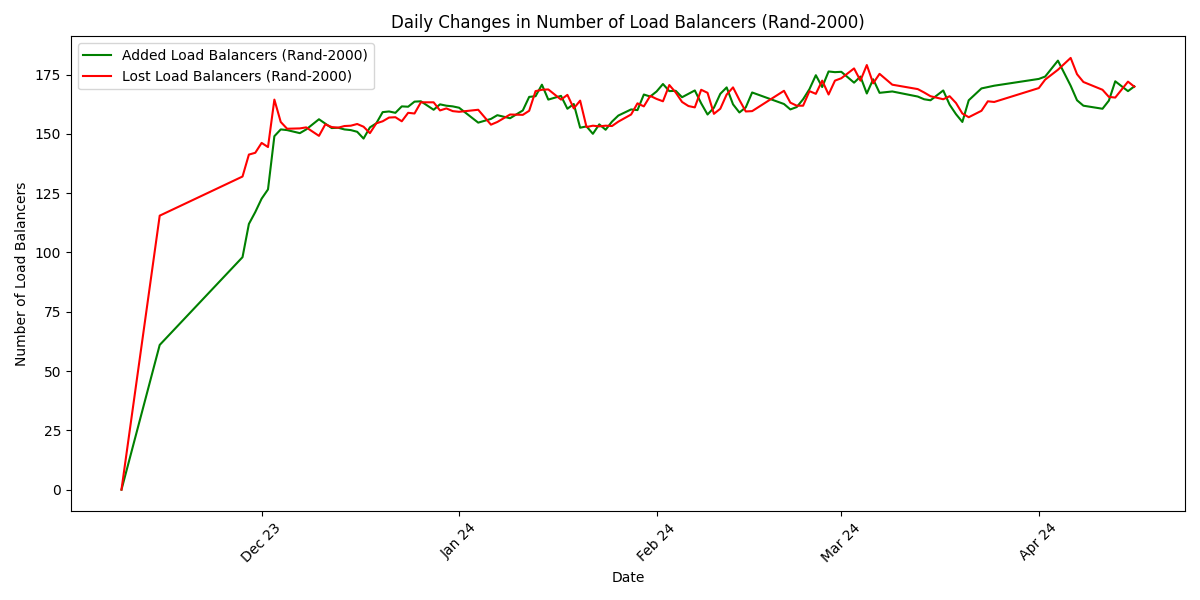
\includegraphics[width=\linewidth]{figures/load_balancer_changes_Rand-2000.png}
    \caption{Daily Changes in Number of Load Balancers for Rand-2000}
    \label{fig:rand2000_changes}
\end{figure}

The analysis shows that load balancers are mostly dynamic and not static, changing over time. Even though the graph for the number of load balancers (fig \ref{fig:scatter_plot_domains}) shows that the number remains relatively stable, the individual load balancers themselves change frequently. This is more evident in the random data because it doesn't consistently target the same paths, leading to higher variability. The average duration of presence further supports this, with load balancers in the Top-2000 dataset averaging 31.10 days, while those in the Rand-2000 dataset average only 12.49 days. This indicates that load balancers adapt to varying network conditions and demands, demonstrating the dynamic nature of network infrastructure.


\subsection{Autonomous Systems}

This subsection presents the AS-specific statistics for both the Top-2000 and Rand-2000 datasets, focusing on daily averages and key metrics related to ASes.

The AS with the most additions per day indicates which AS consistently introduces the most new load balancers. This can reflect the AS's dynamic nature and high level of activity in adjusting its load balancing infrastructure.

The AS with the most removals per day shows which AS frequently removes load balancers. High removal rates can suggest either significant changes in traffic patterns when the load balancing functions are turned off, frequent updates to the network infrastructure when next hops are down, or issues requiring frequent load balancer replacement. It could also be caused by a different route being taken when accessing that website. 

The AS with the longest average duration of presence has load balancers that remain active the longest on average. This indicates a more stable and persistent load balancing infrastructure.

The most consistent AS is present for the most number of times, indicating the AS's load balancers are active across the majority of the observation period, reflecting stability.

The most inconsistent AS is the one that is present for the fewest number of times, suggesting either sporadic use of load balancers or frequent changes in infrastructure. It could also mean that the measurment was a false positive and that it was not truly a load balancer.

The most fluctuating AS has the highest number of load balancer changes, indicating a high level of dynamism in their load balancing strategy, possibly reflecting a need to adapt rapidly to changing traffic conditions or network requirements.

\textbf{Note:} The UCB, US AS was excluded from these statistics as it would consistently be the most reliable AS, given that our tests are conducted from within it.


\subsubsection{Top-2000 Dataset}

For the Top-2000 dataset, observed over 116 days:

\begin{itemize}
    \item \textbf{AS with most additions per day:} CHINANET-BACKBONE No.31, Jin-rong Street, CN, Added: 50.34 per day
    \item \textbf{AS with most removals per day:} CHINANET-BACKBONE No.31, Jin-rong Street, CN, Removed: 50.17 per day
    \item \textbf{AS with longest average duration:} CHINANET-BACKBONE No.31, Jin-rong Street, CN, Average Duration: 159.62 days
    \item \textbf{Most consistent AS:} GOOGLE, US, Present: 75863 times
    \item \textbf{Most inconsistent AS:} AS-NETIA Warszawa 02-822, PL, Present: 1 time
    \item \textbf{Most fluctuating AS:} CHINANET-BACKBONE No.31, Jin-rong Street, CN, Changes: 11660 over 116 days
\end{itemize}

\subsubsection{Rand-2000 Dataset}

For the Rand-2000 dataset, observed over 111 days:

\begin{itemize}
    \item \textbf{AS with most additions per day:} CHINANET-BACKBONE No.31, Jin-rong Street, CN, Added: 29.12 per day
    \item \textbf{AS with most removals per day:} CHINANET-BACKBONE No.31, Jin-rong Street, CN, Removed: 29.40 per day
    \item \textbf{AS with longest average duration:} CHINANET-BACKBONE No.31, Jin-rong Street, CN, Average Duration: 44.09 days
    \item \textbf{Most consistent AS:} GOOGLE, US, Present: 11153 times
    \item \textbf{Most inconsistent AS:} MTS, RU, Present: 1 time
    \item \textbf{Most fluctuating AS:} CHINANET-BACKBONE No.31, Jin-rong Street, CN, Changes: 6495 over 111 days
\end{itemize}

\section{Shared Next Hops Analysis}

This section analyzes the shared next hops between load balancers in both the Top-2000 and Rand-2000 datasets. The objective is to understand the extent to which next hops are shared among multiple load balancers, indicating the presence of common infrastructure and potential load balancing strategies.

\subsection{Top-2000 Dataset}

For the Top-2000 dataset, a total of 9,492 unique next hops were identified. The number of load balancers sharing a next hop ranged from a minimum of 1 to a maximum of 52. On average, each next hop was shared by 5.31 load balancers, with a median value of 2.0. The standard deviation of 6.70 indicates considerable variability in the number of load balancers sharing a next hop. The 75th percentile value was 7.0, and the 95th percentile value was 18.0, showing that a small number of next hops were highly shared among load balancers.

\begin{figure}[h!]
    \centering
    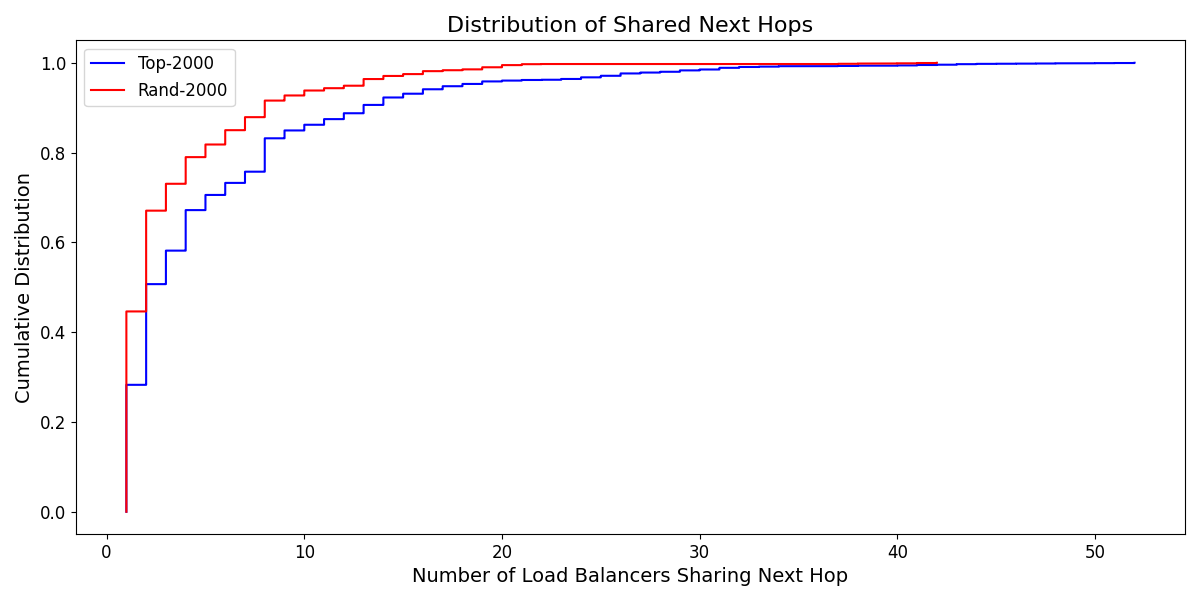
\includegraphics[width=\linewidth]{figures/shared_next_hops_combined.png}
    \caption{Distribution of Shared Next Hops for Top-2000 and Rand-2000}
    \label{fig:shared_next_hops_combined}
\end{figure}

\subsection{Rand-2000 Dataset}

The Rand-2000 dataset revealed 15,797 unique next hops. The number of load balancers sharing a next hop ranged from a minimum of 1 to a maximum of 42. The average number of load balancers sharing a next hop was 3.35, with a median of 2.0. The standard deviation was 4.17, indicating a moderate level of variability. The 75th percentile value was 4.0, and the 95th percentile value was 13.0, suggesting that most next hops were shared by a relatively small number of load balancers.
\newpage

The analysis of shared next hops between load balancers in both datasets highlights key differences and similarities. The Top-2000 dataset shows a higher average number of load balancers sharing a next hop compared to the Rand-2000 dataset. This suggests that the infrastructure supporting the most popular websites is more interconnected and utilizes shared pathways more frequently than the broader, randomly selected websites.

The distribution of shared next hops, as depicted in Figure~\ref{fig:shared_next_hops_combined}, indicates that while most next hops are shared by a small number of load balancers, there are a few next hops that are highly shared, particularly in the Top-2000 dataset. This can be attributed to the reliance on major network infrastructure providers and common routing paths for high-traffic websites.

Overall, the presence of shared next hops signifies the use of common infrastructure, which can enhance efficiency but also poses risks in terms of single points of failure. The variability in the number of shared next hops across both datasets underscores the complexity and dynamic nature of load balancing in different segments of the internet.


\chapter{Layer 3 Load Balancing}
In my research, I found specific load balancers within the Internet2 AS. The Internet2 Network was established to support data-intensive research and advanced campus and cloud computing needs. Internet2's GlobalNOC-developed Router Proxy tool allows users to run commands against network devices, enabling limited testing and viewing active configuration and state information.

These load balancers were accessible via the Internet2 looking glass, allowing deeper analysis of their load balancing techniques. Specifically, we observed that many of the next hops for these load balancers were defined in Cisco Express Forwarding (CEF) tables. The following sections elaborate on the workings of CEF and its role in load balancing.

\section{Network Layer Load Balancing}
Layer 3, known as the network layer, plays a crucial role in load balancing by routing packets based on their IP addresses. This approach focuses on the distribution of traffic across multiple servers without inspecting the packet contents. Unlike higher layers that can make decisions based on the data within the packets, Layer 3 load balancers rely solely on IP addresses and routing tables. This method is efficient and fast but offers less granularity in traffic management, as it does not consider the type or state of the application data. They cannot make decisions based on the content of the traffic, user sessions, or specific application states, which are critical for more advanced load balancing strategies. This means that while Layer 3 load balancers can efficiently manage large volumes of traffic, they lack the detailed traffic management capabilities provided by higher-layer solutions. Nevertheless, technologies like Cisco Express Forwarding (CEF) enhance the efficiency of Layer 3 load balancing by pre-computing forwarding information, ensuring rapid and reliable packet forwarding across the network.

\section{Cisco Express Forwarding (CEF)}

Cisco Express Forwarding (CEF) is a Layer 3 switching technology used to optimize network performance. CEF employs a forwarding information base (FIB) and an adjacency table to expedite the packet forwarding process. The following outlines the critical components and operations of CEF:

\subsection{CEF Components}

\textbf{Forwarding Information Base (FIB)}: The FIB is used by CEF to make IP destination prefix-based switching decisions. It is conceptually similar to a routing table, maintaining a mirror image of the forwarding information in the IP routing table. When routing or topology changes occur, the IP routing table updates, and these changes are reflected in the FIB. The FIB ensures all known routes are covered, eliminating the need for route cache maintenance.

\textbf{Adjacency Table}: The adjacency table complements the FIB by storing Layer 2 addressing information necessary for packet forwarding. Nodes in the network that can reach each other with a single hop across a link layer have their Layer 2 next-hop addresses stored in this table.

\subsection{CEF Operation Modes}

\textbf{Central CEF Mode}: In this mode, both the FIB and adjacency tables reside on the route processor, which performs all express forwarding. This mode is useful when line cards are not available for CEF switching or when features incompatible with distributed CEF switching are needed.

\newpage

\textbf{Distributed CEF (dCEF) Mode}: In dCEF mode, line cards maintain identical copies of the FIB and adjacency tables, enabling them to perform express forwarding independently. This offloads the route processor from being involved in the switching operation, making it particularly efficient for high-performance environments like the Cisco 12000 Series Router.

\subsection{Packet Forwarding Process}

The line cards play a crucial role in forwarding. When a packet arrives, it is placed into input buffers on the receiving line card. The Layer 2/Layer 3 forwarding engine accesses the packet's information and determines its route based on the FIB and adjacency table. The appropriate Layer 2 information is then appended to the packet using data from the adjacency table, and the packet is forwarded to its next-hop destination.

\subsection{Synchronization and Updates}

An Inter-Process Communication (IPC) mechanism ensures synchronization of FIBs and adjacency tables between the route processor and line cards. The GRP (route processor) updates the network routing table and sends forwarding update messages to the FIB tables on the line cards. It also updates the adjacency tables whenever new Layer 2 information is received.

\section{Summary and Findings}

CEF's efficiency in packet forwarding is achieved through its use of optimized data structures (FIB and adjacency tables) and its ability to distribute the forwarding process across different components of the router, particularly in environments where high-speed processing is required. This structured approach allows for rapid and reliable routing of packets across a network, enhancing overall network performance and scalability.

The insights gained from analyzing the Internet2 load balancers revealed that most of the next hops for these load balancers are defined within CEF. This ensures high efficiency and reliability in handling the vast amount of data traffic traversing the Internet2 network. It also means that CEF load balancing is less resource-intensive and does not require any deeper look at the packets.





\begin{figure}[h!]
    \centering
    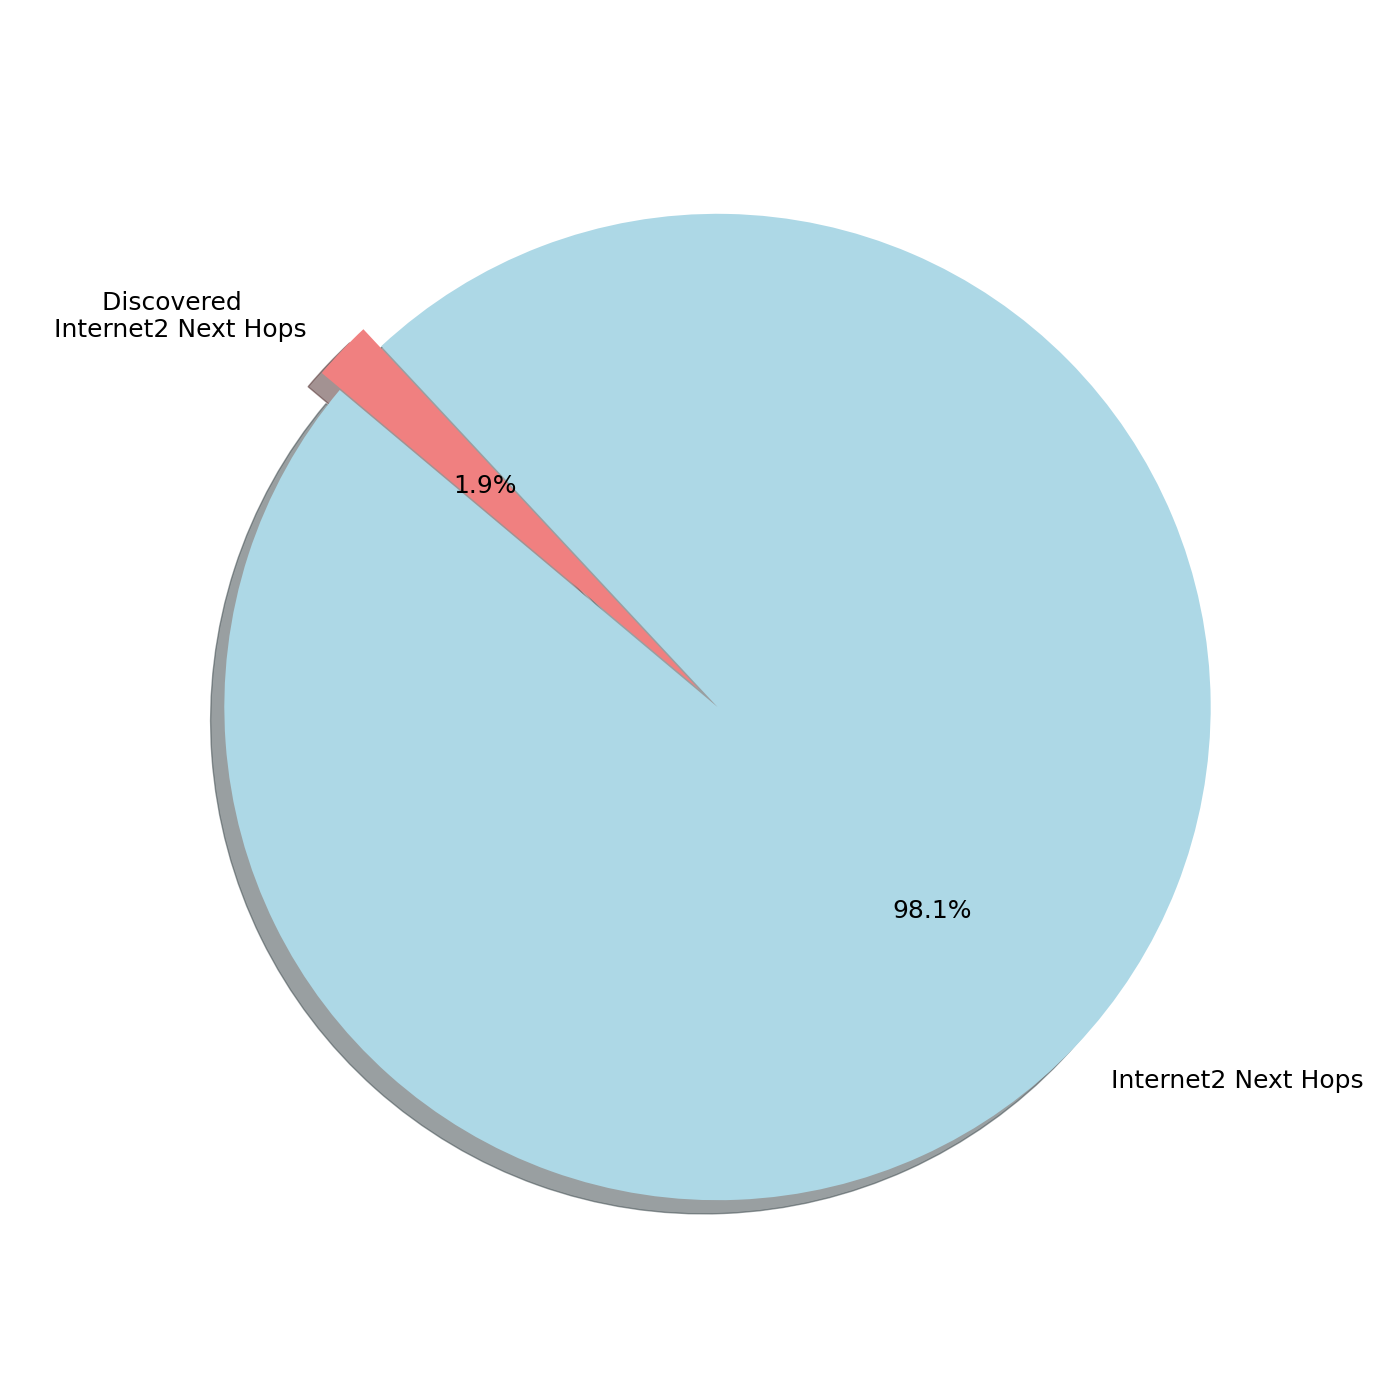
\includegraphics[width =\linewidth]{figures/internet2_next_hops_pie_chart.png}
    \caption{Pie Chart of discovered Internet2 Load Balancers}
    \label{fig:pie_chart_internet2}
\end{figure}

The implementation of load balancing at Layer 3 using CEF highlights the techniques employed to manage network traffic. This leads us to think that a lot of load balancers can be hidden behind the CEF forwarding, which is not usually visible using tools like Paris traceroute. The pie chart \ref{fig:pie_chart_internet2} showing the percentage of next hops found by MDA and the looking glass. Only 1.9\% of the next hops were found using MDA, while the looking glass revealed that 97.9\% were not found by our measurements, either because not enough probes were sent out by MDA, next hops were hidden, or they were not accessible on the specific route taken.
This could mean that a great amount of load balancers are not identifiable using network probing tools and that they are a hidden part of 

\chapter{}
\chapter{This is the Seventh Chapter}
\chapter{This is the Eighth Chapter}


%If you have appendices to your thesis, place them here
\appendix

\chapter{Questionnaire}

\printbibliography[heading=bibintoc]

\end{document}
